\section{Análise de Casos Extremos}

A análise de casos extremos permite identificar padrões nas condições que levam ao sucesso ou falha de diferentes métodos de fusão. Esta seção examina os melhores e piores resultados obtidos, revelando características importantes para seleção apropriada de técnicas.

\subsection{Datasets Mais Desafiadores}

Os cinco conjuntos de imagens que apresentaram maior dificuldade para todos os métodos testados foram:

\begin{enumerate}
    \item \texttt{no_contractor_parking_1}: PSNR médio de 8.51 dB
    \item \texttt{graffiti_car_1}: PSNR médio de 8.73 dB
    \item \texttt{rental_office_1}: PSNR médio de 9.01 dB
    \item \texttt{stop_sign_1}: PSNR médio de 9.74 dB
    \item \texttt{theory_left}: PSNR médio de 9.86 dB
\end{enumerate}

Estes datasets compartilham características que tornam a fusão particularmente desafiadora, como baixo contraste, estruturas altamente repetitivas ou paralaxe pronunciada. A análise detalhada destes casos revela limitações fundamentais das abordagens baseadas em homografia planar global.

\subsection{Padrões de Sucesso e Falha}

Definindo sucesso como PSNR $\geq$ 12.48 dB (quartil superior) e falha como PSNR $\leq$ 9.71 dB (quartil inferior), foram identificados 76 casos de sucesso e 75 casos de falha.

\textbf{Métodos com maior taxa de sucesso:}
\begin{itemize}
    \item Clássico • Blend Hybrid: 5 casos
    \item Clássico • Blend Laplacian: 5 casos
    \item Clássico • Blend Exposure: 5 casos
\end{itemize}

A Figura~\ref{fig:violin_extremos} apresenta a distribuição de PSNR por dataset, comparando métodos clássicos e deep learning.

\begin{figure}[htb]
\centering
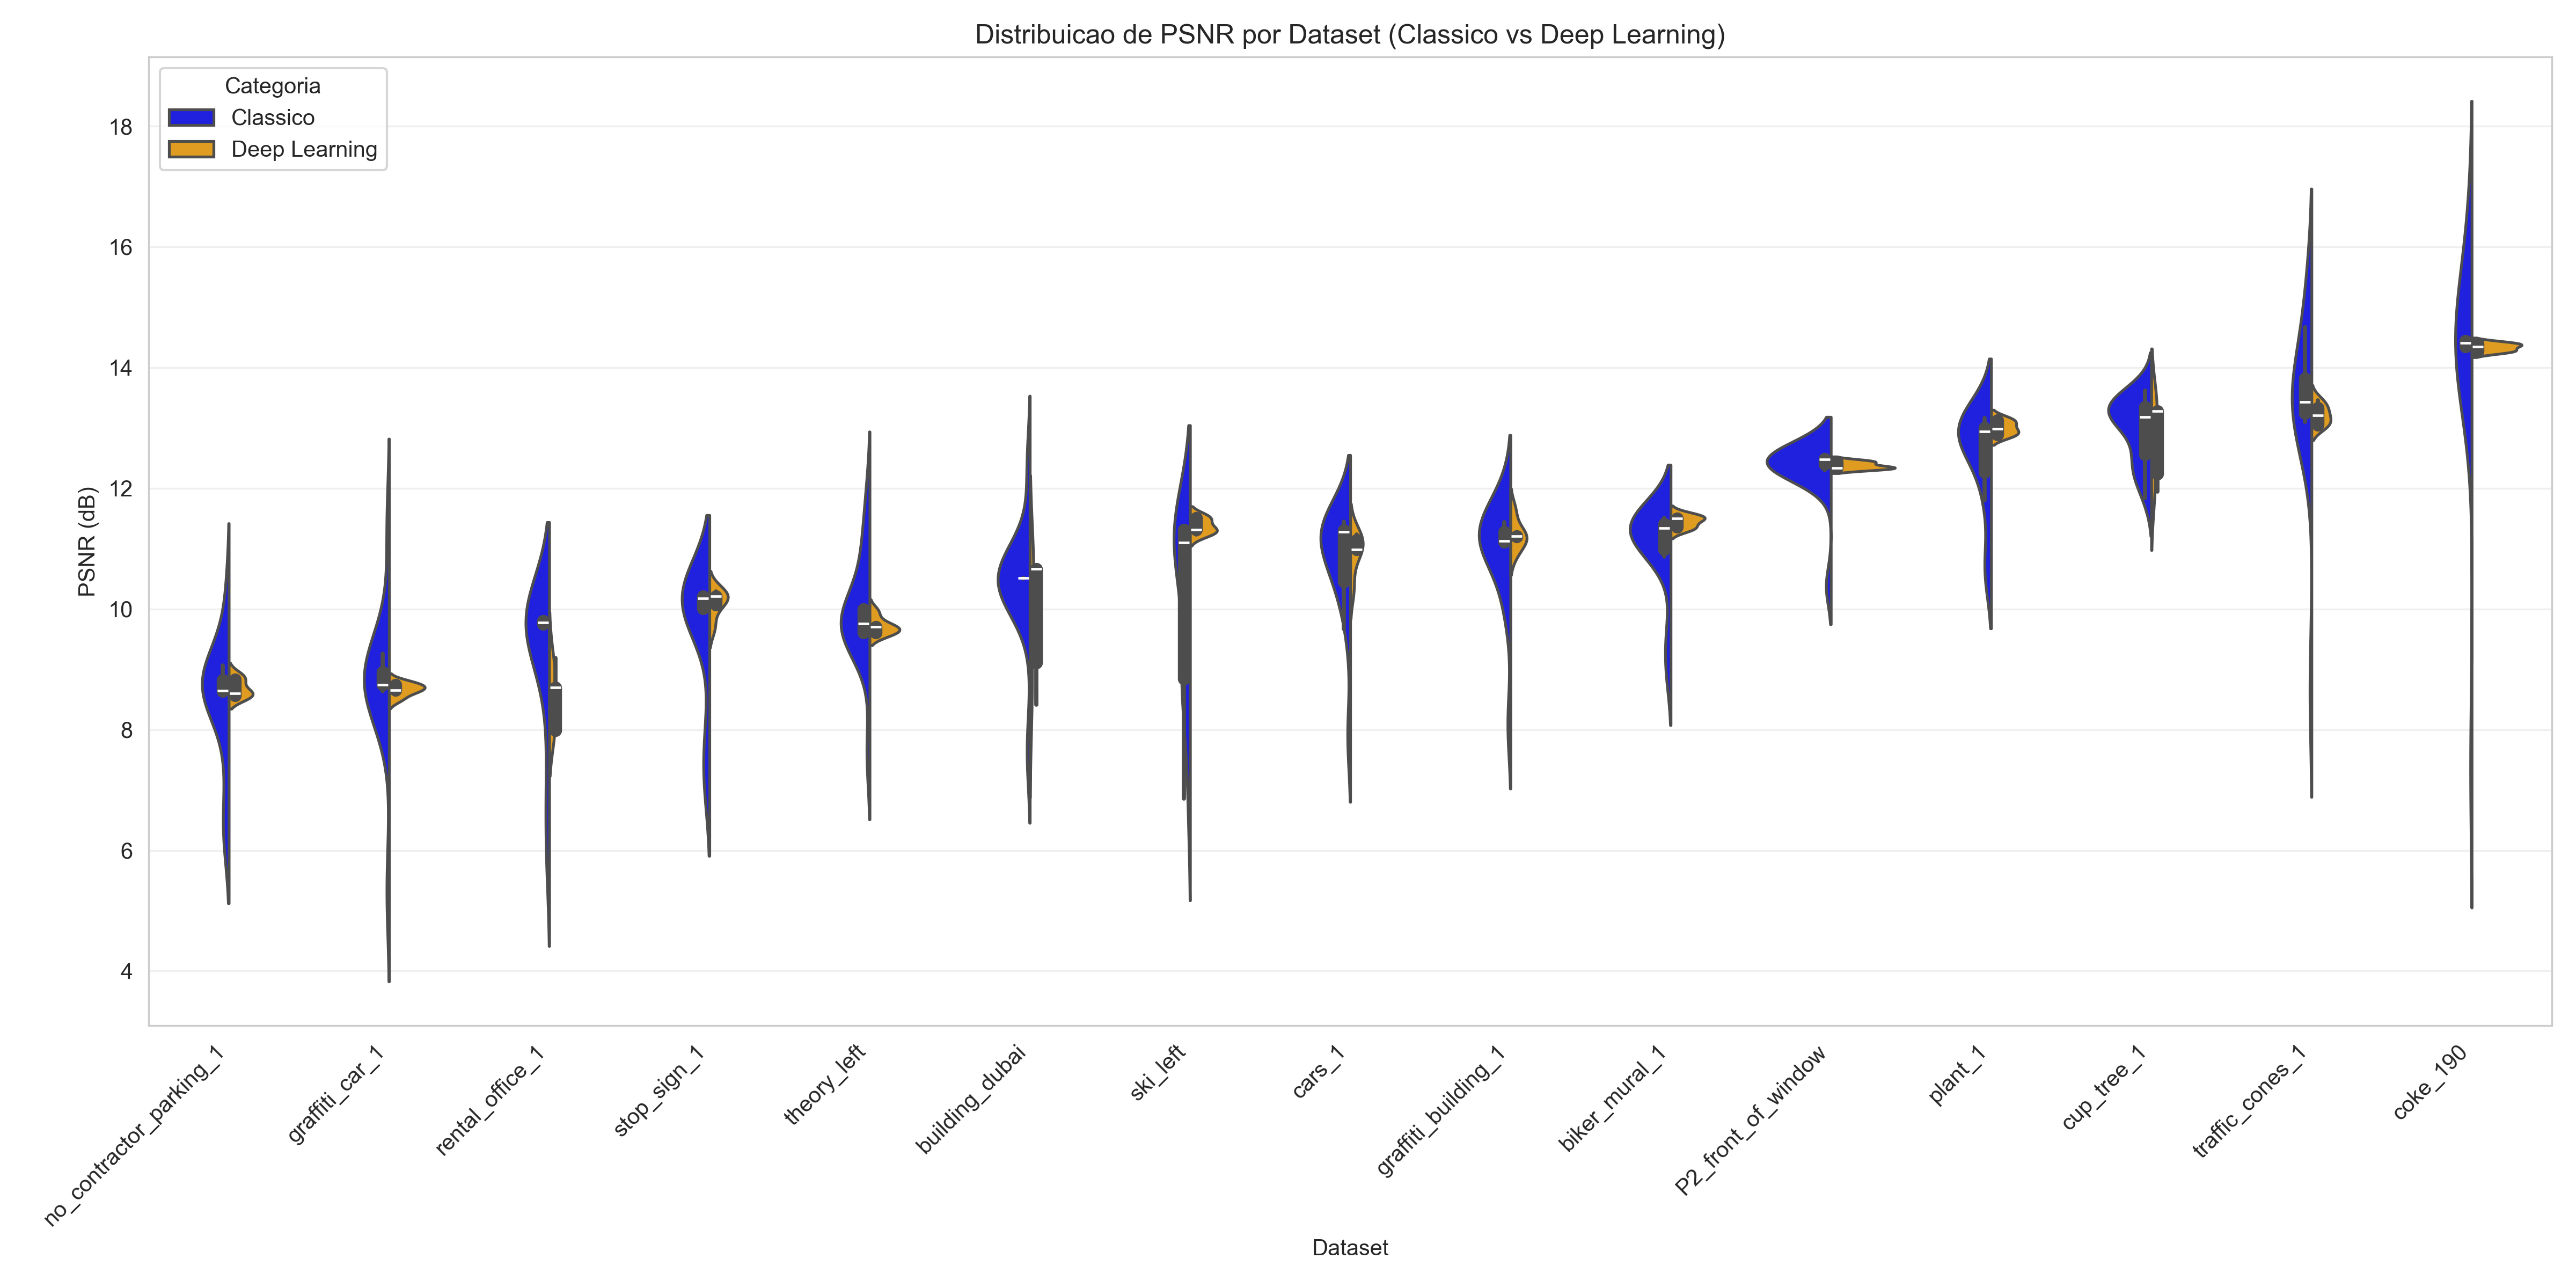
\includegraphics[width=\textwidth]{results/analise_casos_extremos/violin_psnr_por_dataset.png}
\caption{Distribuição de PSNR por dataset: Clássico vs Deep Learning}
\label{fig:violin_extremos}
\fonte{Autoria própria (2025).}
\end{figure}

